\documentclass[tikz, border=1in]{standalone}
\usepackage[utf8]{inputenc}
\usepackage[T1]{fontenc}
\usepackage{tikz}

\usepackage{geometry}




\begin{document}
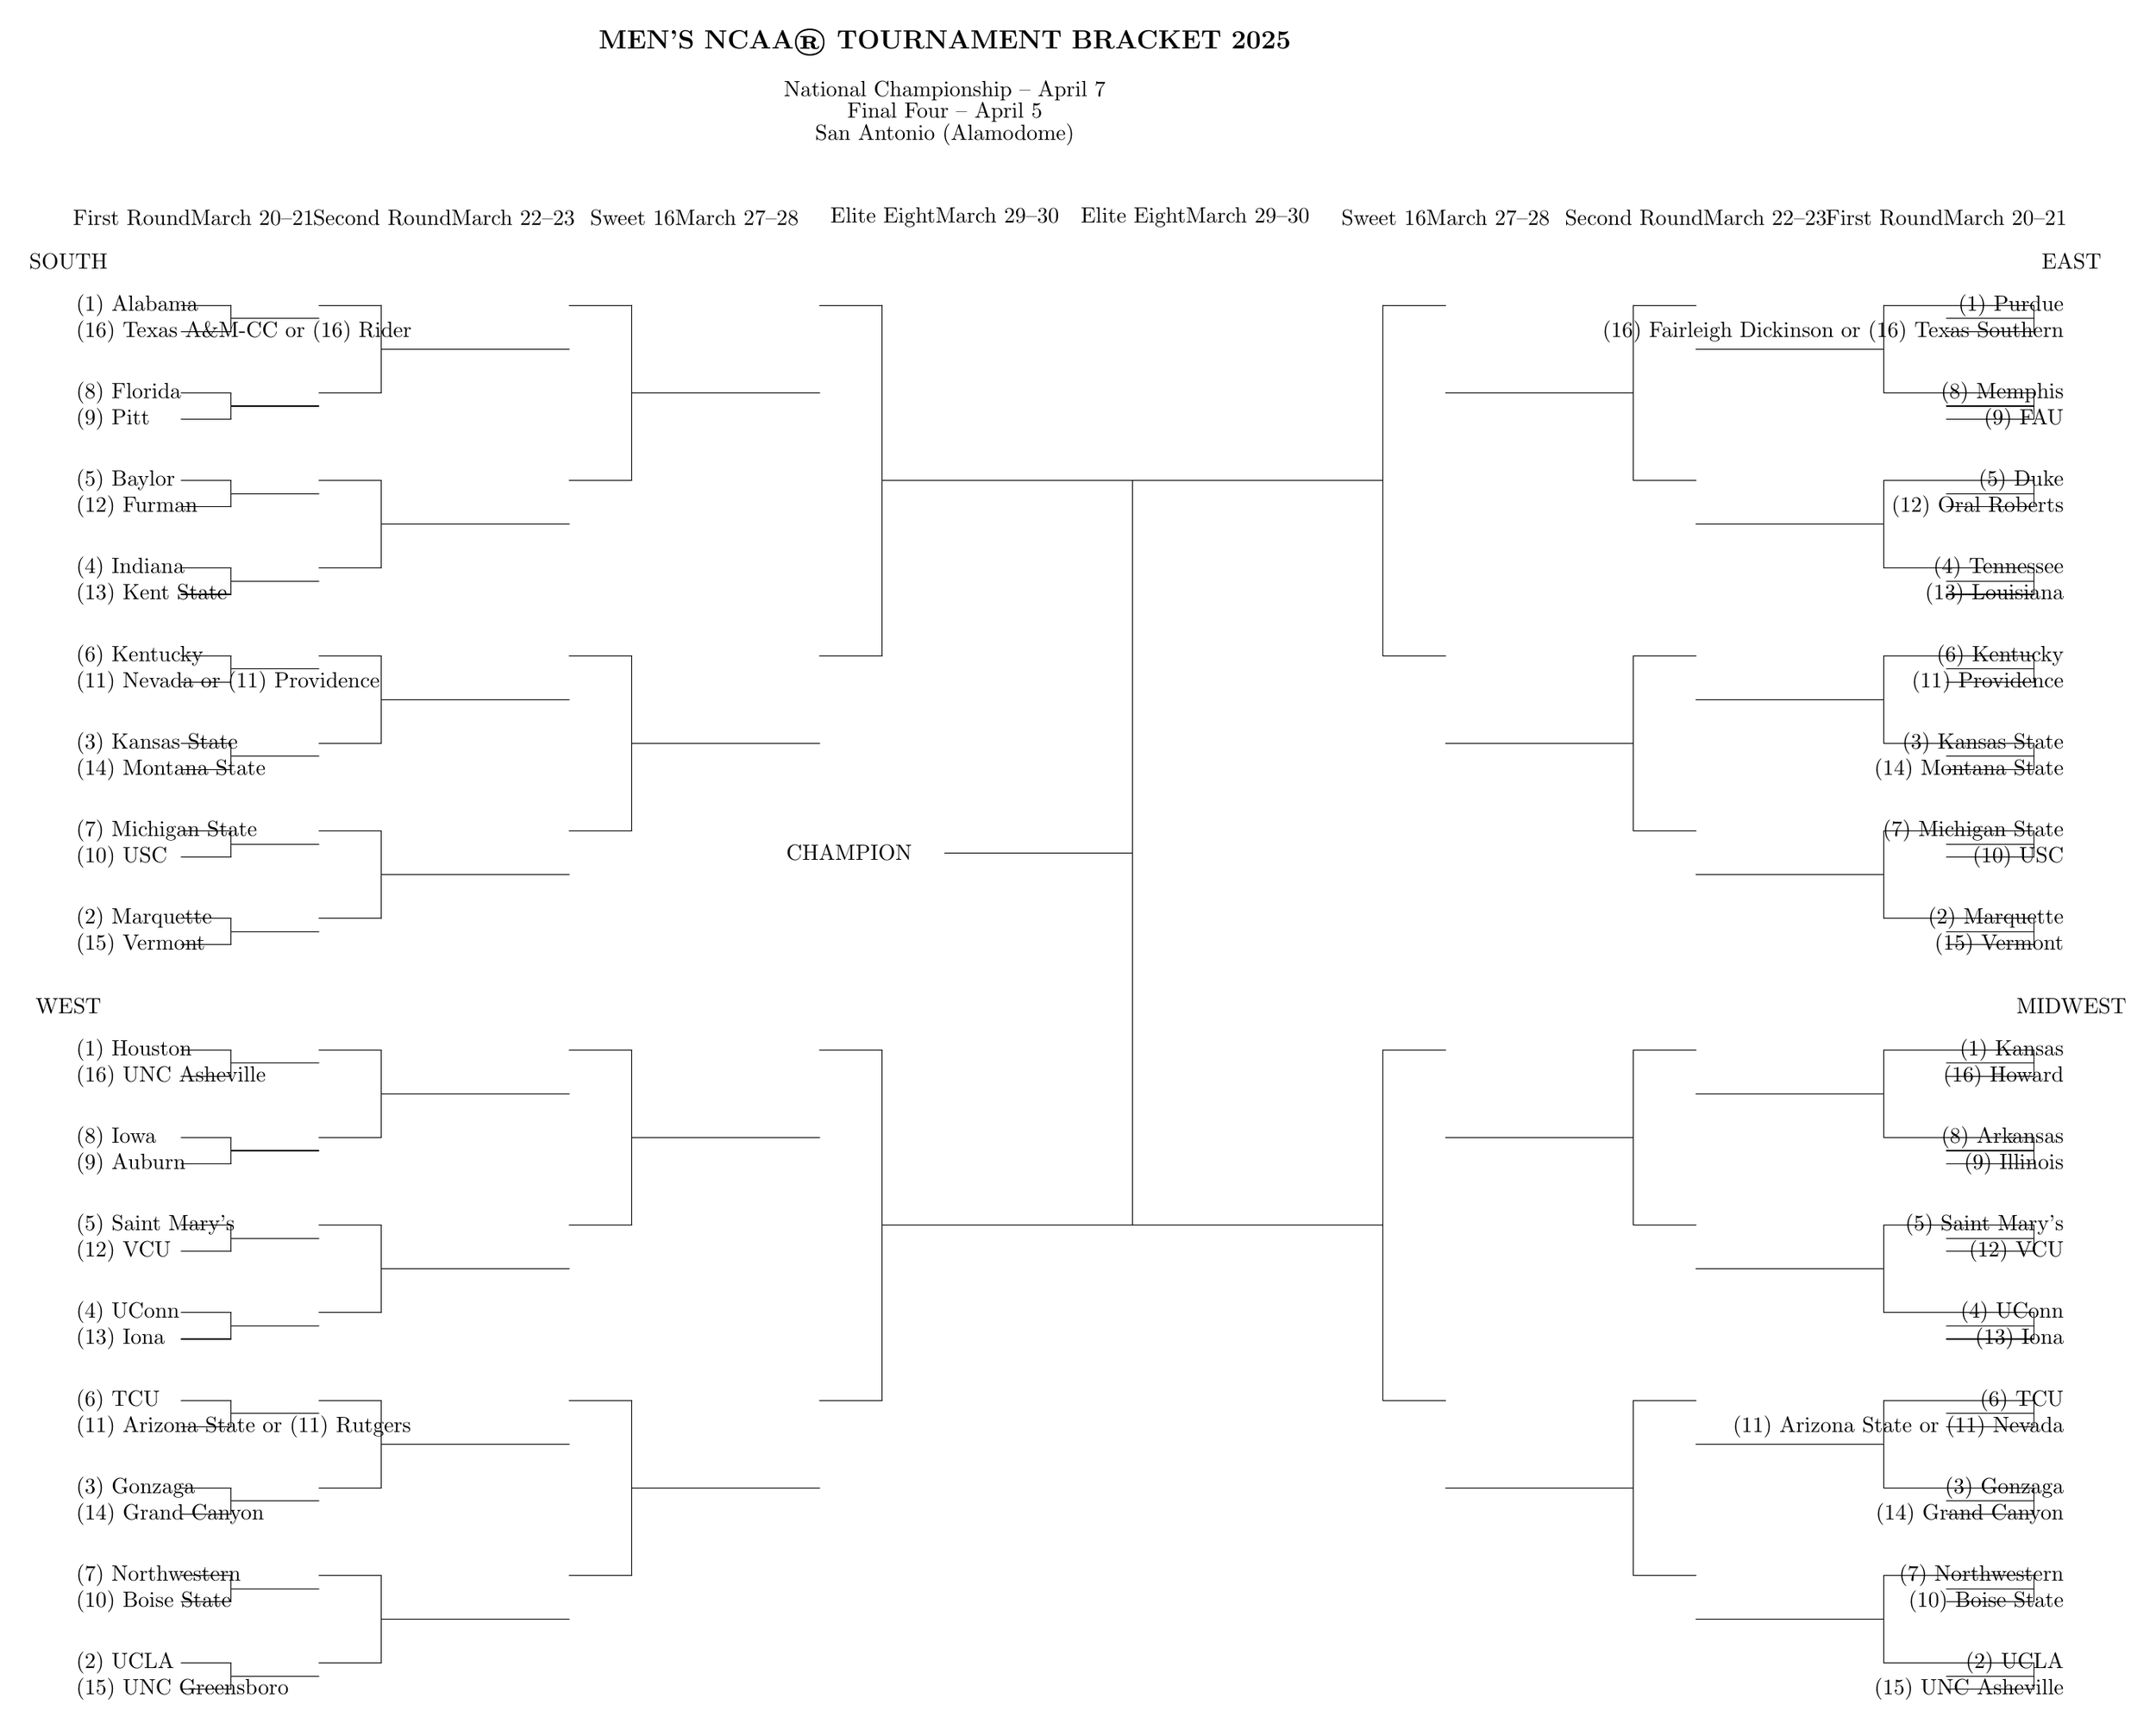
\begin{tikzpicture}[%
        font=\normalsize,
        line cap=round,
        line join=round,
        x=2cm,
        y=0.7cm
    ]

    % -------------------------------------------------
    % Title and headings
    % -------------------------------------------------
    \node[font=\large, align=center] at (7,30) {\textbf{MEN'S NCAA\textregistered{} TOURNAMENT BRACKET 2025}};
    \node at (7,28.9) {National Championship -- April 7};
    \node at (7,28.4) {Final Four -- April 5};
    \node at (7,27.9) {San Antonio (Alamodome)};

    % Round labels (top row)
    \node at (1,26) {First Round\\March 20--21};
    \node at (3,26) {Second Round\\March 22--23};
    \node at (5,26) {Sweet 16\\March 27--28};
    \node at (7,26) {Elite Eight\\March 29--30};
    % Mirror them on the right side
    \node at (9,26) {Elite Eight\\March 29--30};
    \node at (11,26) {Sweet 16\\March 27--28};
    \node at (13,26) {Second Round\\March 22--23};
    \node at (15,26) {First Round\\March 20--21};

    % -------------------------------------------------
    % LEFT SIDE BRACKETS
    % -------------------------------------------------
    % Regions: South (top-left), West (bottom-left)

    % ============= SOUTH REGION =============
    \node[font=\normalsize, text depth=0] at (0,25) {SOUTH};

    % -- Round of 64 pairings (x=0), seeds + teams
    % We place them from top (y=24) downward
    % Each "matchup" is two lines. We'll connect them to Round of 32 (x=2).
    % You can tweak y offsets to match your image more precisely.

    % (1) Alabama vs (16) Texas A&M-CC / Rider
    \node[anchor=west] at (0,24) {(1) Alabama};
    \node[anchor=west] at (0,23.4) {(16) Texas A\&M-CC or (16) Rider};

    % (8) Florida vs (9) Pitt
    \node[anchor=west] at (0,22) {(8) Florida};
    \node[anchor=west] at (0,21.4) {(9) Pitt};

    % (5) Baylor vs (12) Furman
    \node[anchor=west] at (0,20) {(5) Baylor};
    \node[anchor=west] at (0,19.4) {(12) Furman};

    % (4) Indiana vs (13) Kent State
    \node[anchor=west] at (0,18) {(4) Indiana};
    \node[anchor=west] at (0,17.4) {(13) Kent State};

    % (6) Kentucky vs (11) Nevada / Providence
    \node[anchor=west] at (0,16) {(6) Kentucky};
    \node[anchor=west] at (0,15.4) {(11) Nevada or (11) Providence};

    % (3) Kansas State vs (14) Montana State
    \node[anchor=west] at (0,14) {(3) Kansas State};
    \node[anchor=west] at (0,13.4) {(14) Montana State};

    % (7) Michigan State vs (10) USC
    \node[anchor=west] at (0,12) {(7) Michigan State};
    \node[anchor=west] at (0,11.4) {(10) USC};

    % (2) Marquette vs (15) Vermont
    \node[anchor=west] at (0,10) {(2) Marquette};
    \node[anchor=west] at (0,9.4) {(15) Vermont};

    % -- Lines from Round of 64 (x=0) to Round of 32 (x=2)
    % We draw them in pairs, bridging the two lines of each matchup to one line in Round 2
    \foreach \i in {0,...,7} {
            % Y positions for the top/bottom line of each pairing
            \pgfmathsetmacro{\ytop}{24 - 2*\i}
            \pgfmathsetmacro{\ybot}{\ytop - 0.6}
            \pgfmathsetmacro{\ymid}{(\ytop + \ybot)/2}
            % horizontal lines from x=0.9 to x=1.3
            \draw (0.9,\ytop) -- (1.3,\ytop);
            \draw (0.9,\ybot) -- (1.3,\ybot);
            % vertical line from ybot to ytop at x=1.3
            \draw (1.3,\ybot) -- (1.3,\ytop);
            % single line to round 2 at x=2
            \draw (1.3,\ymid) -- (2,\ymid);
        }

    % -- Round of 32 (x=2) to Sweet 16 (x=4)
    % We'll have 4 pairings. Each pairing merges two from the prior round.
    % The top pairing merges seeds (1/16 vs 8/9), etc.
    % We'll store midpoints in an array-like approach:
    \foreach \j in {0,...,3} {
            \pgfmathsetmacro{\ytop}{24 - 4*\j}
            \pgfmathsetmacro{\ybot}{\ytop - 2}
            \pgfmathsetmacro{\ymid}{(\ytop + \ybot)/2}
            % horizontal lines from x=2 to x=2.5
            \draw (2,\ytop) -- (2.5,\ytop);
            \draw (2,\ybot) -- (2.5,\ybot);
            % vertical line at x=2.5
            \draw (2.5,\ybot) -- (2.5,\ytop);
            % line out to x=4
            \draw (2.5,\ymid) -- (4,\ymid);
        }

    % -- Sweet 16 (x=4) to Elite 8 (x=6)
    % We have 2 matchups
    \foreach \k in {0,...,1} {
            \pgfmathsetmacro{\ytop}{24 - 8*\k}
            \pgfmathsetmacro{\ybot}{\ytop - 4}
            \pgfmathsetmacro{\ymid}{(\ytop + \ybot)/2}
            \draw (4,\ytop) -- (4.5,\ytop);
            \draw (4,\ybot) -- (4.5,\ybot);
            \draw (4.5,\ybot) -- (4.5,\ytop);
            \draw (4.5,\ymid) -- (6,\ymid);
        }

    % -- Elite 8 (x=6) to Final Four (x=8)
    % We have 1 matchup
    \draw (6,24) -- (6.5,24);
    \draw (6,16) -- (6.5,16);
    \draw (6.5,16) -- (6.5,24);
    \draw (6.5,20) -- (8,20);

    % ============= WEST REGION (below SOUTH) =============
    \node[font=\normalsize, text depth=0] at (0,8) {WEST};

    % Round of 64 for West (similar pattern, we just shift y-values down)
    % We'll do them from y=7 down in steps
    \foreach \i/\teamA/\teamB in {
    0/{(1) Houston}/{(16) UNC Asheville},
    1/{(8) Iowa}/{(9) Auburn},
    2/{(5) Saint Mary's}/{(12) VCU},
    3/{(4) UConn}/{(13) Iona},
    4/{(6) TCU}/{(11) Arizona State or (11) Rutgers},
    5/{(3) Gonzaga}/{(14) Grand Canyon},
    6/{(7) Northwestern}/{(10) Boise State},
    7/{(2) UCLA}/{(15) UNC Greensboro}
    }{
    \pgfmathsetmacro{\ytop}{7 - 2*\i}
    \pgfmathsetmacro{\ybot}{\ytop - 0.6}
    \node[anchor=west] at (0,\ytop) {\teamA};
    \node[anchor=west] at (0,\ybot) {\teamB};
    % bracket lines to Round of 32
    \draw (0.9,\ytop) -- (1.3,\ytop);
    \draw (0.9,\ybot) -- (1.3,\ybot);
    \draw (1.3,\ybot) -- (1.3,\ytop);
    \draw (1.3,{(\ytop+\ybot)/2}) -- (2,{(\ytop+\ybot)/2});
    }

    % Round of 32 for West
    \foreach \j in {0,...,3} {
            \pgfmathsetmacro{\ytop}{7 - 4*\j}
            \pgfmathsetmacro{\ybot}{\ytop - 2}
            \draw (2,\ytop) -- (2.5,\ytop);
            \draw (2,\ybot) -- (2.5,\ybot);
            \draw (2.5,\ybot) -- (2.5,\ytop);
            \draw (2.5,{(\ytop+\ybot)/2}) -- (4,{(\ytop+\ybot)/2});
        }

    % Sweet 16 for West
    \foreach \k in {0,...,1} {
            \pgfmathsetmacro{\ytop}{7 - 8*\k}
            \pgfmathsetmacro{\ybot}{\ytop - 4}
            \draw (4,\ytop) -- (4.5,\ytop);
            \draw (4,\ybot) -- (4.5,\ybot);
            \draw (4.5,\ybot) -- (4.5,\ytop);
            \draw (4.5,{(\ytop+\ybot)/2}) -- (6,{(\ytop+\ybot)/2});
        }

    % Elite 8 (West) to Final Four
    \draw (6,7) -- (6.5,7);
    \draw (6,-1) -- (6.5,-1);
    \draw (6.5,-1) -- (6.5,7);
    \draw (6.5,3) -- (8,3);

    % -------------------------------------------------
    % RIGHT SIDE BRACKETS
    % -------------------------------------------------
    % Regions: East (top-right), Midwest (bottom-right)

    % ============= EAST REGION =============
    \node[font=\normalsize, text depth=0] at (16,25) {EAST};

    % Round of 64 (mirroring on x ~ 16)
    % We'll label seeds as in the example bracket
    \foreach \i/\teamA/\teamB in {
    0/{(1) Purdue}/{(16) Fairleigh Dickinson or (16) Texas Southern},
    1/{(8) Memphis}/{(9) FAU},
    2/{(5) Duke}/{(12) Oral Roberts},
    3/{(4) Tennessee}/{(13) Louisiana},
    4/{(6) Kentucky}/{(11) Providence},
    5/{(3) Kansas State}/{(14) Montana State},
    6/{(7) Michigan State}/{(10) USC},
    7/{(2) Marquette}/{(15) Vermont}
    }{
    \pgfmathsetmacro{\ytop}{24 - 2*\i}
    \pgfmathsetmacro{\ybot}{\ytop - 0.6}
    \node[anchor=east] at (16,\ytop) {\teamA};
    \node[anchor=east] at (16,\ybot) {\teamB};
    % lines in Round of 64
    \draw (15.1,\ytop) -- (15.7,\ytop);
    \draw (15.1,\ybot) -- (15.7,\ybot);
    \draw (15.7,\ybot) -- (15.7,\ytop);
    \draw (15,\ytop) -- (15.1,\ytop);  % short horizontal to visually match left side
    \draw (15,\ybot) -- (15.1,\ybot);
    \draw (15.7,{(\ytop+\ybot)/2}) -- (15,{(\ytop+\ybot)/2});
    }

    % Round of 32 (mirroring from x=15 to x=13)
    \foreach \j in {0,...,3} {
            \pgfmathsetmacro{\ytop}{24 - 4*\j}
            \pgfmathsetmacro{\ybot}{\ytop - 2}
            \draw (15,\ytop) -- (14.5,\ytop);
            \draw (15,\ybot) -- (14.5,\ybot);
            \draw (14.5,\ybot) -- (14.5,\ytop);
            \draw (14.5,{(\ytop+\ybot)/2}) -- (13,{(\ytop+\ybot)/2});
        }

    % Sweet 16 (x=13 to x=11)
    \foreach \k in {0,...,1} {
            \pgfmathsetmacro{\ytop}{24 - 8*\k}
            \pgfmathsetmacro{\ybot}{\ytop - 4}
            \draw (13,\ytop) -- (12.5,\ytop);
            \draw (13,\ybot) -- (12.5,\ybot);
            \draw (12.5,\ybot) -- (12.5,\ytop);
            \draw (12.5,{(\ytop+\ybot)/2}) -- (11,{(\ytop+\ybot)/2});
        }

    % Elite 8 (x=11 to x=9)
    \draw (11,24) -- (10.5,24);
    \draw (11,16) -- (10.5,16);
    \draw (10.5,16) -- (10.5,24);
    \draw (10.5,20) -- (9,20);

    % ============= MIDWEST REGION (below EAST) =============
    \node[font=\normalsize, text depth=0] at (16,8) {MIDWEST};

    \foreach \i/\teamA/\teamB in {
    0/{(1) Kansas}/{(16) Howard},
    1/{(8) Arkansas}/{(9) Illinois},
    2/{(5) Saint Mary's}/{(12) VCU},
    3/{(4) UConn}/{(13) Iona},
    4/{(6) TCU}/{(11) Arizona State or (11) Nevada},
    5/{(3) Gonzaga}/{(14) Grand Canyon},
    6/{(7) Northwestern}/{(10) Boise State},
    7/{(2) UCLA}/{(15) UNC Asheville}
    }{
    \pgfmathsetmacro{\ytop}{7 - 2*\i}
    \pgfmathsetmacro{\ybot}{\ytop - 0.6}
    \node[anchor=east] at (16,\ytop) {\teamA};
    \node[anchor=east] at (16,\ybot) {\teamB};
    \draw (15.1,\ytop) -- (15.7,\ytop);
    \draw (15.1,\ybot) -- (15.7,\ybot);
    \draw (15.7,\ybot) -- (15.7,\ytop);
    \draw (15,\ytop) -- (15.1,\ytop);
    \draw (15,\ybot) -- (15.1,\ybot);
    \draw (15.7,{(\ytop+\ybot)/2}) -- (15,{(\ytop+\ybot)/2});
    }

    \foreach \j in {0,...,3} {
            \pgfmathsetmacro{\ytop}{7 - 4*\j}
            \pgfmathsetmacro{\ybot}{\ytop - 2}
            \draw (15,\ytop) -- (14.5,\ytop);
            \draw (15,\ybot) -- (14.5,\ybot);
            \draw (14.5,\ybot) -- (14.5,\ytop);
            \draw (14.5,{(\ytop+\ybot)/2}) -- (13,{(\ytop+\ybot)/2});
        }

    \foreach \k in {0,...,1} {
            \pgfmathsetmacro{\ytop}{7 - 8*\k}
            \pgfmathsetmacro{\ybot}{\ytop - 4}
            \draw (13,\ytop) -- (12.5,\ytop);
            \draw (13,\ybot) -- (12.5,\ybot);
            \draw (12.5,\ybot) -- (12.5,\ytop);
            \draw (12.5,{(\ytop+\ybot)/2}) -- (11,{(\ytop+\ybot)/2});
        }

    \draw (11,7) -- (10.5,7);
    \draw (11,-1) -- (10.5,-1);
    \draw (10.5,-1) -- (10.5,7);
    \draw (10.5,3) -- (9,3);

    % -------------------------------------------------
    % FINAL FOUR + CHAMPIONSHIP (Center)
    % -------------------------------------------------
    % Left winners come in at x=8, top y=20 (South), bottom y=3 (West)
    % Right winners come in at x=9, top y=20 (East), bottom y=3 (Midwest)

    % We can unify them around x=8.5 or so
    % Semifinal lines (top match: y=20 from left, y=20 from right)
    \draw (8,20) -- (8.5,20);
    \draw (9,20) -- (8.5,20);

    % Semifinal lines (bottom match: y=3 from left, y=3 from right)
    \draw (8,3) -- (8.5,3);
    \draw (9,3) -- (8.5,3);

    % Vertical line for the Final Four matchups
    \draw (8.5,3) -- (8.5,20);

    % Championship line from the midpoint (y=11.5 or so) to x=7
    \draw (8.5,11.5) -- (7,11.5);

    % Node for CHAMPION
    \node[anchor=east, font=\normalsize] at (6.8,11.5) {CHAMPION};

\end{tikzpicture}
\end{document}
